\chapter{Background Subtraction}
Background Subtraction bzw. Foreground Detection besch\"aftigen sich mit der Detektion von sich bewegenden Objekten in der Bildverarbeitung. Um Objekte durch ihre Bewegung erkennen zu k\"onnen ist es notwendig, eine Folge von Bildern in ihrem zeitlichen Verlauf zu analysieren und so \"Anderungen feststellen zu k\"onnen. Das Ziel der Background Subtraction ist es, die Dimension des Bildes zu reduzieren. In vielen Anwendungen, insbesondere im Bereich Stra\ss{}enverkehr und Fahrerassistenz, sind nur dynamische Objekte relevant. Um nicht die knappe Rechenzeit auf statischen Hintergrund zu verschwenden wird so versucht die relevanten Bildausschnitte zu extrahieren und nur diese zu analysieren.
Ergebnis der Background Subtraction ist im Allgemeinen eine bin\"are Maske \(B \in \{0,1\}^{m \times n} \). Pixel welche dynamische Objekte enthalten haben dabei den Wert \(1\), alle anderen Pixel sind Hintergrund und erhalten den Wert \(0\). Auf diese Weise kann die Maske logisch auf das Originalbild \(I \in \mathbb{R}^{m \times n} \) angewendet werden um den Vordergrund \(F \) zu erhalten:
\begin{equation*}
 F_{ij} = 
 \begin{cases}
  I_{ij} & B_{ij}=1 \\
  0 & B_{ij}=0
 \end{cases}
\end{equation*}

\section{Frame Difference}

Die Methoden die mit Mitteln der Frame Difference arbeiten bilden die Differenz aus dem zu analysierenden Bild \(I^t \in \mathbb{R}^{m \times n} \) mit einem Referenzbild \(R^t \in \mathbb{R}^{m \times n}\). Die so entstandene Differenz \( D^t \) wird anschlie\ss{}end mittels Threshold auf \"Anderungen \"uberpr\"uft:
\begin{eqnarray*}
 D_{ij}^t &=& |R_{ij}^t-I_{ij}^t| \\
 B_{ij}^t &=& D_{ij}^t > Threshold
\end{eqnarray*}
Das Referenzbild kann hierbei ein statisches, zuvor festgelegtes Bild sein oder es wird das zeitlich vorangegangene Bild als Referenz verwendet. Die Wahl des Schwellwerts bestimmt wie stark die Abweichung sein muss, damit Pixel als Vordergrund klassifiziert werden. Bei zu hohem Schwellwert werden eventuell dynamische Pixel nicht als solche erkannt, bei zu geringem Schwellwert ist das Gegenteil der Fall und es kommt h\"aufig zu Rauschen im Bild. Allgemein stellt das Rauschen beim Bilden der Frame Difference ein gro\ss{}es Problem dar. Um hierbei stabilere Ergebnisse zu erhalten wird in \cite{background_threeframediff} vorgeschlagen, statt nur zwei Bilder die Differenz aus je zwei aufeinander folgenden Bildern zu verwenden und die Ergebnisse logisch zu verkn\"upfen:
\begin{equation*}
 B_{ij}^t =
 \begin{cases}
  1 & (D_{ij}^{t-1} > Threshold) \cap (D_{ij}^t > Threshold) = 1 \\
  0 & sonst
 \end{cases}
\end{equation*}

\section{Weitere Methoden}

Es existieren eine Reihe weiterer Verfahren, welche sich wesentlich an der Bildung der Frame Difference orientieren. Dazu z\"ahlt beispielsweise der Mittelwertfilter, welcher als Referenzbild den Mittelwert der letzten \(l\) Bilder berechnet:
\begin{equation*}
 R_{ij}^t=\frac{1}{l}\sum_{k=1}^l I_{ij}^{t-k}
\end{equation*}
Einen \"ahnlichen Ansatz verwendet das Gau\ss{}verfahren. Hierbei werden die letzten \(l\) Pixelwerte durch eine Gau\ss{}verteilung angen\"ahert:
\begin{equation}
 R_{ij}
\end{equation}


\begin{figure}
 \centering
 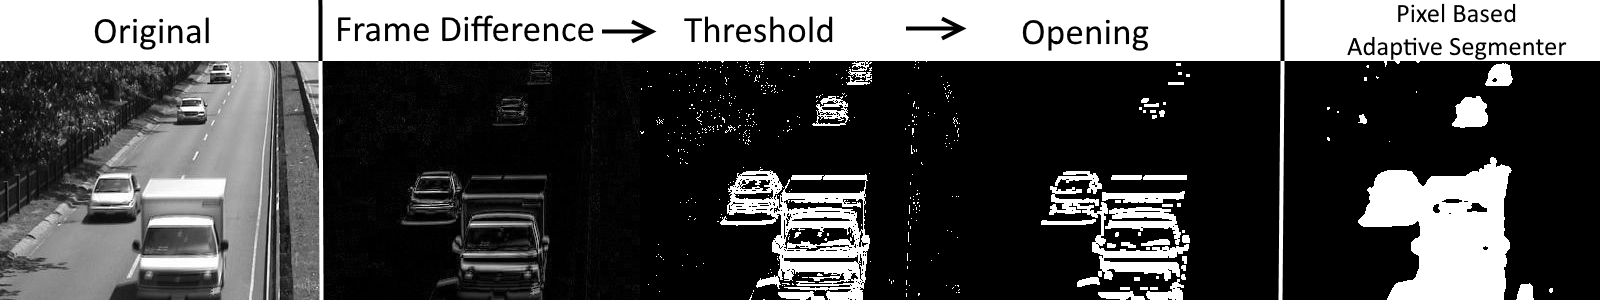
\includegraphics[width=1\textwidth]{media/background/background_text.png}
 \caption{Background Subtraction - Original, Frame Difference, PBAS}
 \label{fig:background_comparison}
\end{figure}
